\documentclass{beamer}

\usefonttheme{professionalfonts} % using non standard fonts for beamer
\usefonttheme{serif} % default family is serif

\usepackage{hyperref}

%\usepackage{minted}

\usepackage{animate}

\usepackage{graphicx}

\def\Put(#1,#2)#3{\leavevmode\makebox(0,0){\put(#1,#2){#3}}}

\usepackage{color}

\usepackage{tikz}

\usepackage{amssymb}

\usepackage{enumerate}


\newcommand\blfootnote[1]{%

  \begingroup

  \renewcommand\thefootnote{}\footnote{#1}%

  \addtocounter{footnote}{-1}%

  \endgroup

}

\makeatletter

%%%%%%%%%%%%%%%%%%%%%%%%%%%%%% Textclass specific LaTeX commands.

 % this default might be overridden by plain title style

 \newcommand\makebeamertitle{\frame{\maketitle}}%

 % (ERT) argument for the TOC

 \AtBeginDocument{%

   \let\origtableofcontents=\tableofcontents

   \def\tableofcontents{\@ifnextchar[{\origtableofcontents}{\gobbletableofcontents}}

   \def\gobbletableofcontents#1{\origtableofcontents}

 }

%%%%%%%%%%%%%%%%%%%%%%%%%%%%%% User specified LaTeX commands.

\usetheme{Malmoe}

% or ...

\useoutertheme{infolines}

\addtobeamertemplate{headline}{}{\vskip2pt}



\setbeamercovered{transparent}

% or whatever (possibly just delete it)

\makeatother

\begin{document}
\title[DCEL report]{RIDIR Report}
\author[AC]{Andres Calderon}
\institute[Fall'19]{University of California, Riverside}
\makebeamertitle
\newif\iflattersubsect

\AtBeginSection[] {
    \begin{frame}<beamer>
    \frametitle{Outline} 
    \tableofcontents[currentsection]  
    \end{frame}
    \lattersubsectfalse
}

\AtBeginSubsection[] {
    \begin{frame}<beamer>
    \frametitle{Outline} 
    \tableofcontents[currentsubsection]  
    \end{frame}
}

\begin{frame}{Working on partitioning issue}
    \begin{itemize}
        \item GeoSpark partitioners retrive a small number of partitions when deal with polygons
        \item I have tried some alternatives:
        \begin{itemize}
            \item StandardQuadTree: the low-level data structure in GeoSpark.  Allows to set parameters as maxItemsPerZone and maxLevel but even setting minimal values the number of partitions is small.
            \item Simba, Stark and JTS Quadtree: There are no direct access to the geometry of the Partitioner's cells.  We should understand and modify the source code.
            \item Workaround: Force a grow up on those partitions of the GeoSpark's quadtree with a large number of edges. I already have a prototype but it still need to test the performance.
        \end{itemize}
    \end{itemize}
\end{frame}

\begin{frame}{Test - CA\_districts 2010 dataset}
    \centering 
    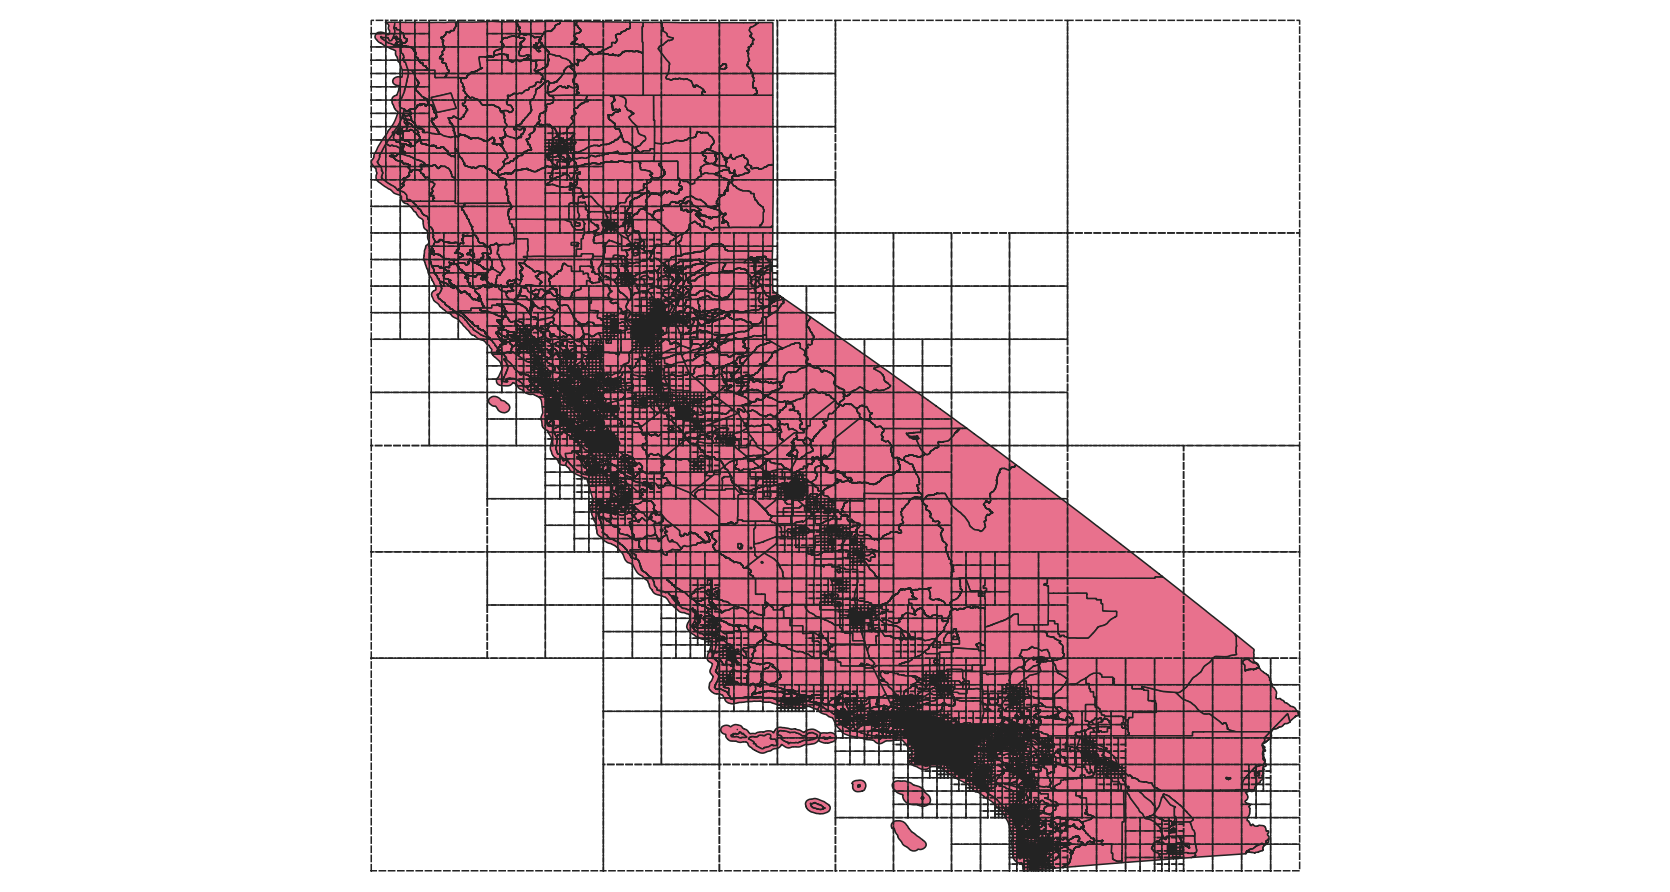
\includegraphics[width=\linewidth]{figures/CA_ForceGrowUp} 
\end{frame}

\begin{frame}{Focus on bug during integration and additional tests}
    \begin{itemize}
        \item It is related to the precision of Polygon's coordinates.  Some polygon's sections are not touching by a very small margin.  
        \item Fixed on Phili datasets by truncating to 6 decimal places.
        \item Run experiments with CA\_districts datasets 2000 and 2010. Merged DCEL is done but the overlay operations still fails for errors during the merging stage.
        \item Checking the correct coordinate system and precision.
    \end{itemize}
\end{frame}

\begin{frame}{Test - CA\_districs dataset - 2000 vs 2010}
    \centering 
    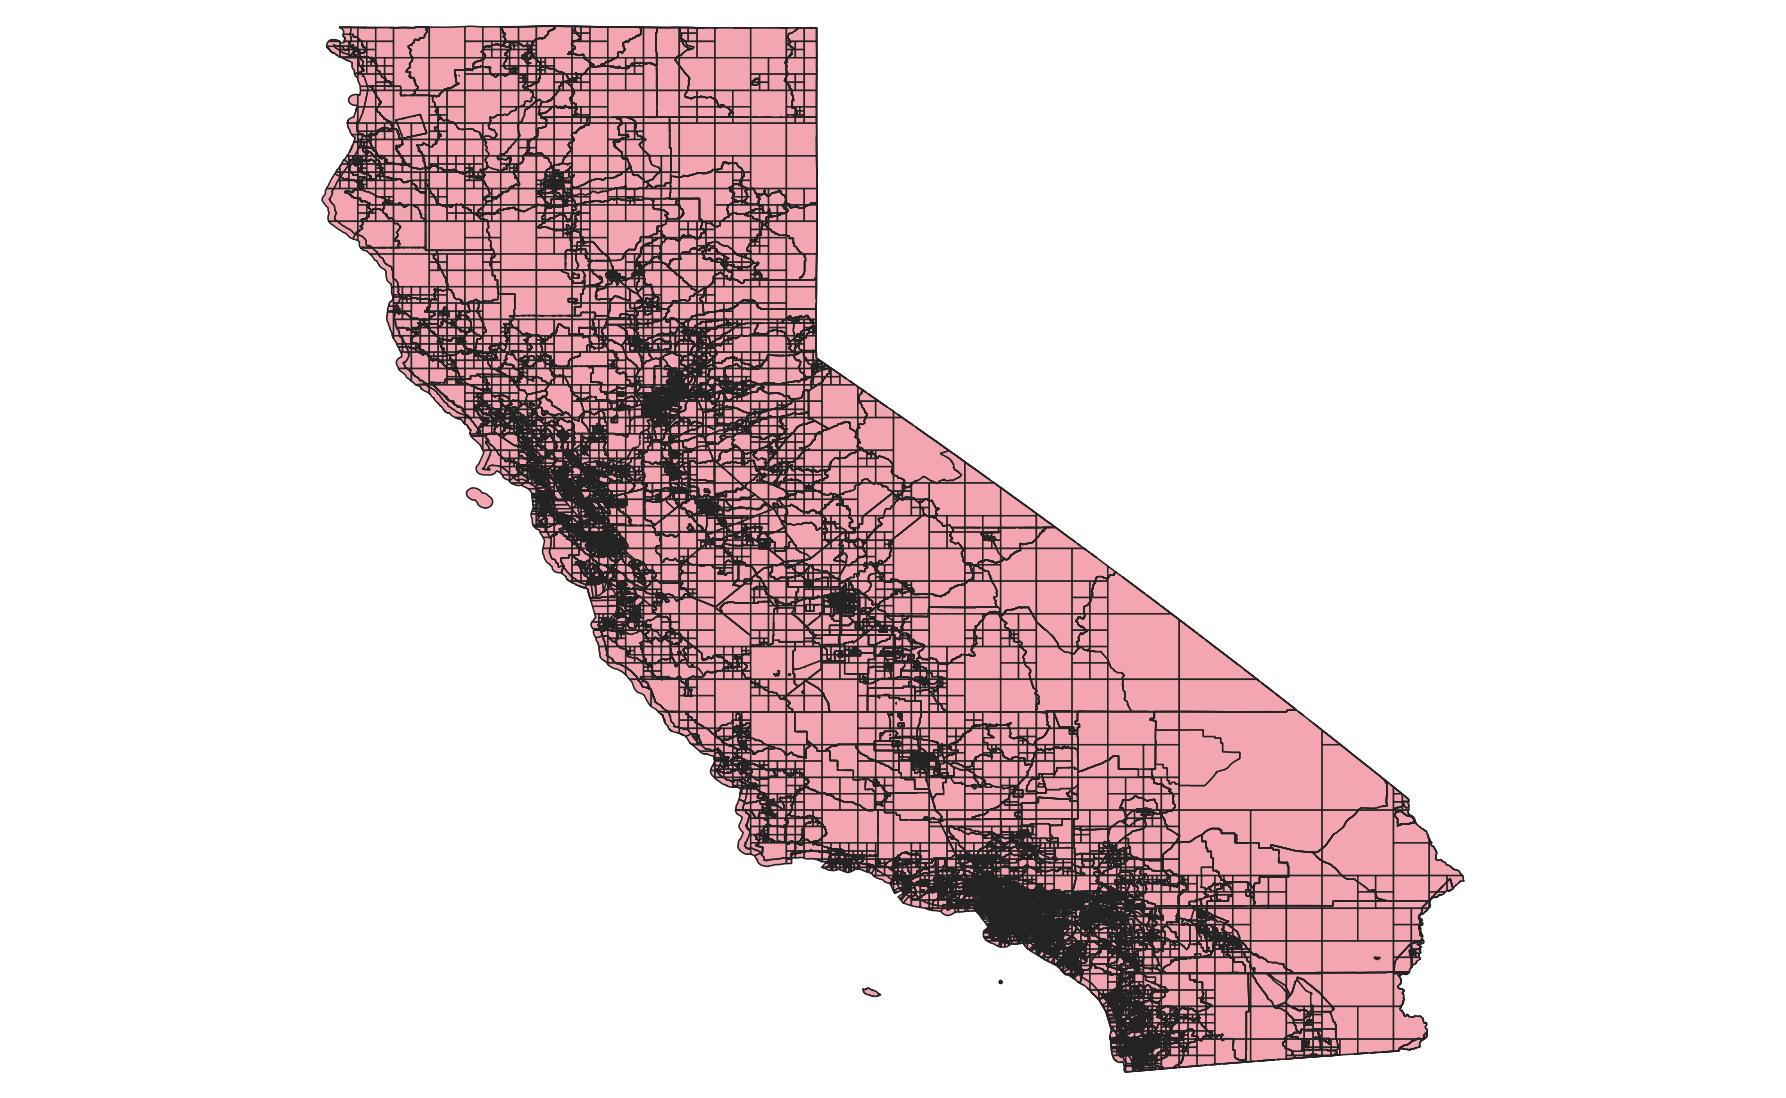
\includegraphics[width=\linewidth]{figures/CA_DCELMerged} 
\end{frame}

\begin{frame}{Output -CA\_districs dataset - 2000 vs 2010}
    \centering 
    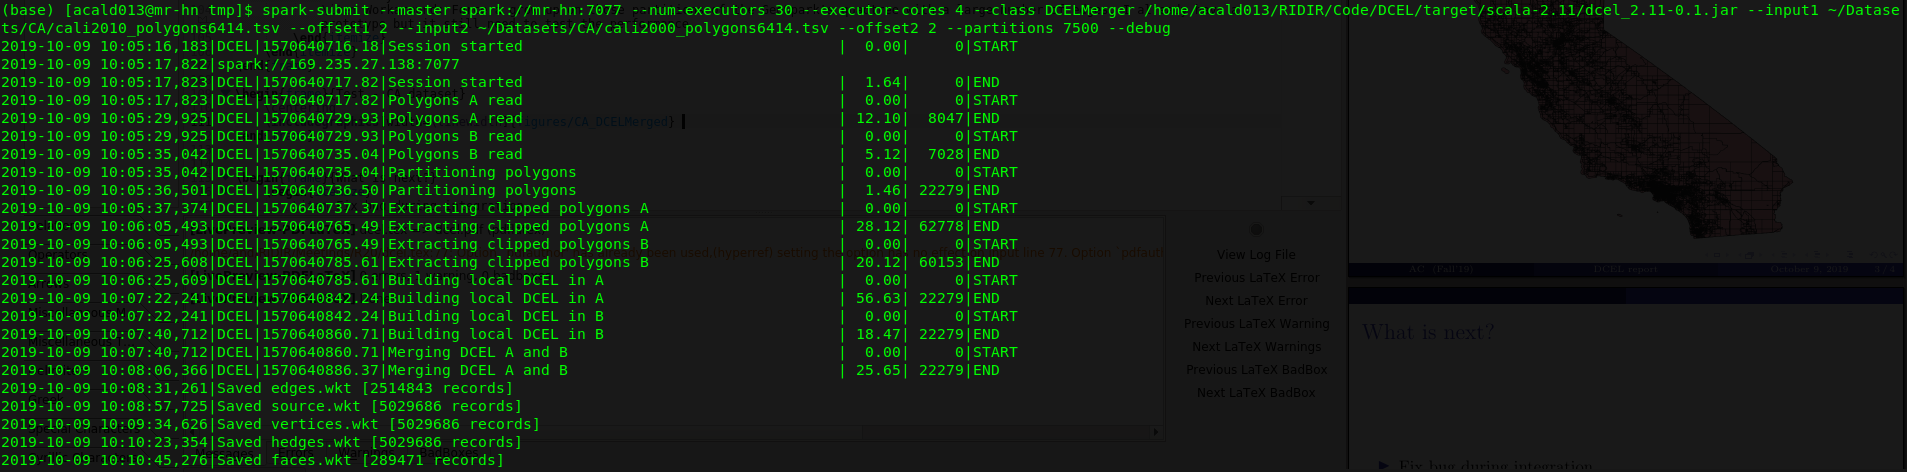
\includegraphics[width=\linewidth]{figures/CA_Test_Output} 
\end{frame}

\begin{frame}{What is next?}
    \begin{itemize}
        \item Decide and integrate the partition strategy.
        \item Work on CA\_districts datasets 2000 vs 2010 issues.
        \item Check support for multipolygons.
    \end{itemize}
\end{frame}

\end{document}
